
\chapter{単一Elasticsearchノードをクラスタ化する前に行うデータ移行}
\label{chap:third}

\section{緒言}
本章では単一Elasticsearchノードをクラスタ化する前に行うデータ移行について述べる.

\section{Elasticsearchの概要}
Elasticsearchは, 分散処理に対応した全文検索エンジンである. 主な特徴は, 以下の通りである.

\begin{itemize}
  \item 高速な検索性能: ビッグデータなどの巨大で複雑なデータの集合にも対応可能
  \item 部分一致検索が可能: 検索キーワードの一部に一致するドキュメントも検索可能
  \item ほぼリアルタイムの検索: ドキュメントにインデックスを付けてから検索可能になるまで約1秒程度
  \item スケーラビリティ: サーバー数を増やすことで, 検索性能と処理能力を拡張可能
\end{itemize}

これらの特徴から, Elasticsearchは, 以下のような用途に適している.

\begin{itemize}
  \item ログ分析: Webサイトやアプリケーションのログから, アクセス状況やエラー情報を分析する
  \item セキュリティインテリジェンス: ネットワークやシステムから, セキュリティ脅威を検知する
  \item ビジネス分析: 顧客データや販売データから, トレンドや傾向を分析する
\end{itemize}

\section{Kibanaの概要}

Kibanaは, Elasticsearchに保存されたデータを可視化するためのツールである. 主な特徴は, 以下の通りである.

\begin{itemize}
  \item 直感的な操作性: ドラッグ&ドロップで簡単に可視化を作成できる
  \item 豊富な可視化機能: グラフ, 表, 地図など, さまざまな可視化機能を提供
  \item 高度なフィルタリング機能: 条件を指定して, データを詳細に絞り込むことができる
\end{itemize}

これらの特徴から, Kibanaは, 以下のような用途に適している.

\begin{itemize}
  \item ログ分析: Webサイトやアプリケーションのログから, アクセス状況やエラー情報を可視化する
  \item セキュリティインテリジェンス: ネットワークやシステムから, セキュリティ脅威を可視化する
  \item ビジネス分析: 顧客データや販売データから, トレンドや傾向を可視化する
\end{itemize}

% \section{学内ゾーンで稼働しているElasticsearchシステムの状況}
% 学内ゾーンでは, 単一ノードで稼働する133.71.106.168のElasticsearchと, 133.71.106.170, 133.71.106.141, 133.71.106.136のElasticsearchノードによって構成されたElasticsearchクラスタが稼働している.

% 133.71.106.168のElasticsearchには, CO\textsubscript{2}濃度監視システムによって計測されたデータとLEAFの運行日誌に関するデータが保存されている.

% \section{CO\textsubscript{2}濃度監視システムの概要}
% CO\textsubscript{2}濃度監視システムとは共通講義棟 C, 工学部 5 号館,工学部 4 号館の各講義室(計 24 部屋)の CO2 濃度を学内ネットワーク内の web サイトで閲覧することができるシステムである.

\section{データ移行対象のElasticsearchインデックスについて}

133.71.106.168で稼働している単一ノードのElasticsearchに保存されたCO\textsubscript{2}データとLEAFの運行日誌に関するデータを, Elasticsearchクラスタへ移行する.

\subsection{CO\textsubscript{2}データ}

CO\textsubscript{2}データが保存されたインデックスは, インデックス名にco2という文字列が含まれているため, co2という文字列を含む全てのインデックスを移行対象とする.

\subsection{LEAFの運行日誌に関するデータ}

LEAFの運行日誌に関するデータが保存されたインデックスは以下の2つである.

\begin{itemize}
  \item movement\_diary
  \item movement\_diary01
\end{itemize}

上記のインデックスに保存されているデータについて説明する.

以下にmovement\_diaryとmovement\_diary01のドキュメントの違いを列挙する.

\begin{enumerate}
  \item driverフィールド:
        \begin{itemize}
          \item movement\_diaryのドキュメントでは, driverフィールドは文字列である.
          \item movement\_diary01のドキュメントでは, driverフィールドは配列で, その中に文字列と2つのnull値が含まれている.
        \end{itemize}
        
  \item ``destination''フィールド:
        \begin{itemize}
          \item movement\_diaryのドキュメントでは, ``destination''フィールドは単一の文字列である.
          \item movement\_diary01のドキュメントでは, ``destination''フィールドは配列で, その中に2つの文字列が含まれている.
        \end{itemize}
        
  \item ``charge\_place''フィールド:
        \begin{itemize}
          \item movement\_diaryのドキュメントには, ``charge\_place''フィールドは存在しない.
          \item movement\_diary01のドキュメントでは, ``charge\_place''フィールドが追加されているが, その値は空文字列である.
        \end{itemize}
        
  \item ``battery\_rate''フィールド:
        \begin{itemize}
          \item movement\_diaryのドキュメントには, ``battery\_rate''フィールドは存在しない.
          \item movement\_diary01のドキュメントでは, ``battery\_rate''フィールドが追加されており, その値は数値である.
        \end{itemize}
        
  \item ``battery\_rate\_distance''フィールド:
        \begin{itemize}
          \item movement\_diaryのドキュメントには, ``battery\_rate\_distance''フィールドは存在しない.
          \item movement\_diary01のドキュメントでは, ``battery\_rate\_distance''フィールドが追加されており, その値は数値である.
        \end{itemize}
\end{enumerate}

上述したドキュメントの違いより, movement\_diary01はmovement\_diaryのもつ全ての情報を保持しており, 更にmovement\_diaryにはないフィールドを持っている. 更に, movement\_diaryとmovement\_diary01のドキュメント数は等しく, すべてのドキュメントのタイムスタンプが一致しているため, movement\_diary01インデックスのみ移行する.

\section{CO\textsubscript{2}データの移行手順ついて}
Elasticsearchに保存されたCO\textsubscript{2}データには, 計測時刻, 部屋番号, 部屋の気温, CO\textsubscript{2}濃度などの情報が含まれている.

CO\textsubscript{2}デーのタ移行を行うに当たって, 計測時刻と部屋番号の組み合わせが重複しているデータが一部存在しているため, 重複データを削除した上でデータを移行する必要がある. そこで一度, 移行元のElasticSearchサーバーのデータをローカルマシンにエクスポートして, 重複データを取り除いた上で, 移行先のElasticSearchサーバーにデータをインサートする.

\subsection{データのエクスポート}
移行元のElasticSearchサーバーのデータのローカルマシンへのエクスポートには, elasticdumpライブラリを使用して, JSON形式でエクスポートした.その際, co2という文字列を含むインデックスのデータのみをエクスポートした.

\subsection{データの重複削除}
重複データの削除はSQLiteデータベースを用いて行った.

SQLiteは, 軽量で自己完結型のデータベースエンジンである. SQLiteは以下の特徴を持っている.

\begin{itemize}
  \item 軽量: SQLiteは非常に小さく, リソースの少ない環境でも動作する.
  \item 自己完結型: データベースが単一のファイルとして存在し, 外部の依存関係がない.
  \item 
        トランザクション: SQLiteはACIDトランザクションをサポートしており, データの整合性を保つ. 
  \item 
        フリーかつオープンソース: SQLiteはパブリックドメインに属し, 誰でも自由に使用, 変更, 配布可能である.
\end{itemize}

SQLiteでは, 複合主キーを使って複数のテーブルカラムの組み合わせを一意の識別子として扱うことができる. これにより, 同じ組み合わせのデータを重複して挿入しようとした場合, データベースエンジンがコンフリクトエラーを発生させ, 重複データの挿入を阻止する. そのため, 今回の重複データ削除には適していると判断した.

今回使用したSQLiteでは, 部屋番号(number)と計測時刻(utctime)を複合主キーとして設定した. 以下のリスト\ref{sc1}, リスト\ref{sc2}に示すように, 移行元のElasticSearchサーバーに保存されているco2インデックスのドキュメントは, ドキュメントの持つフィールドが統一されておらず, 一部のセンサー情報が存在しないドキュメントが存在する. そのため, SQLiteへのデータ挿入時にコンフリクトエラーが発生した場合は, 既存のレコードと挿入しようとしたレコードを比較し, 既存レコードの値がNULLであるカラムにおいて, 挿入しようとしているレコードの値が非NULLである場合は, 既存レコードのカラムの値を更新するようにした. これにより, 重複データ削除時に一部のセンサー情報などが欠けてしまう問題を解決した.

\begin{lstlisting}[caption=\_sourceフィールドのメンバー数が少ないドキュメント, label=sc1]
{
  "_index": "co2_e411",
  "_type": "_doc",
  "_id": "nEi2nnoB2-iFXnrMOobM",
  "_score": 1,
  "_source": {
      "utctime": "2020-10-09T05:09:06+00:00",
      "number": "E411",
      "PPM": "481",
      "data": "Thingspeak"
  }
}
  \end{lstlisting}

\begin{lstlisting}[caption=\_sourceフィールドのメンバー数が多いドキュメント, label=sc2]
{
  "_index": "co2_e411",
  "_type": "_doc",
  "_id": "YKBqU4QBugDzeydA2gyi",
  "_score": 1,
  "_source": {
      "RH": 26.98,
      "PPM": 423,
      "JPtime": "2022-11-06T22:45:30.080925",
      "ip": "172.23.68.19/16",
      "utctime": "2022-11-06T13:45:30.080895",
      "TEMP": 24.47,
      "index_name": "co2_e411",
      "ms": "",
      "number": "E411"
  }
}
    \end{lstlisting}

\subsection{データのインポート}
重複データ削除を行った後のデータが保存されているSQLiteからすべてのレコードを読み出して, 移行先のElasticSearchサーバーにインサートした.

その際, pythonのelasticsearchライブラリを使用し, co2\_modbusという名前のインデックスに保存した.

\section{一度目のデータ移行で移行できなかったCO\textsubscript{2}データの移行について}

2023年5月中旬頃に, 実装したデータ移行プログラムを使用してElasticsearchクラスタへCO\textsubscript{2}データの移行を行った. しかし, CO\textsubscript{2}濃度監視システムの開発と運用を担当している高木君が, 計測データのインサート先を, Elasticsearchクラスタに変更したのが2023年7月中旬頃であった. このため, 2023年5月中旬から2023年7月中旬までの間の約2ヶ月間のCO\textsubscript{2}データがElasticSearchクラスタに移行出来ていなかった. そこで, 追加の移行作業を行った.

移行方法は以下のとおりである.

\begin{enumerate}
  \item まず, 2023年5月中旬に移行した際の全ての移行データの中で最も最新のutctimeフィールドの値を検索する.
        % \begin{itemize}
        %   \item 検索した結果, 2023年5月中旬に移行した際の全移行データの中で最も新しいutctimeは「2023-05-16T05:48:30.081305」であった.
        % \end{itemize}
  \item 次に, Elasticsearchクラスタに対して, CO\textsubscript{2}濃度監視システムからインサートした全データの中で最も古いutctimeフィールドの値を検索する.
        % \begin{itemize}
        %   \item 検索した結果, CO\textsubscript{2}濃度監視システムからインサートされた全データの中で最も古いutctimeは「2023-07-20T07:15:39.314008」であった.
        % \end{itemize}
  \item co2という文字列を含むインデックスに保存された2023年5月1日0時0分0秒以降のutctimeを持つドキュメントを, elasticdumpライブラリを使用して移行元Elasticsearchサーバーからローカルマシンにエクスポートする.
  \item 部屋番号(number)と計測時刻(utctime)の組み合わせがユニークになるようSQLiteを用いて, エクスポートしたデータの重複削除を行う.
  \item ステップ1, 2で得られたutctimeの範囲に含まれるutctimeを持つドキュメントのみになるよう重複削除後のデータをフィルタリングする.
  \item フィルタリング後のデータを移行先ElasticSearchクラスタにインサートする.
\end{enumerate}

上記に手順に従い, 追加のデータ移行を行った.

\section{KibanaによるCO\textsubscript{2}データの可視化}

計2回のCO\textsubscript{2}データを移行した後のco2\_modbusインデックスについて, 横軸を計測時刻(utctime)とし, 縦軸をPPM, RH, 気温としてそれぞれプロットしたものを図 \ref{p12} 〜 図 \ref{p14}に示す.

\begin{figure}[H]
  \hspace*{-2cm} % ここで左に2cmずらす
  \centering % center環境の代わりにこちらを使用
  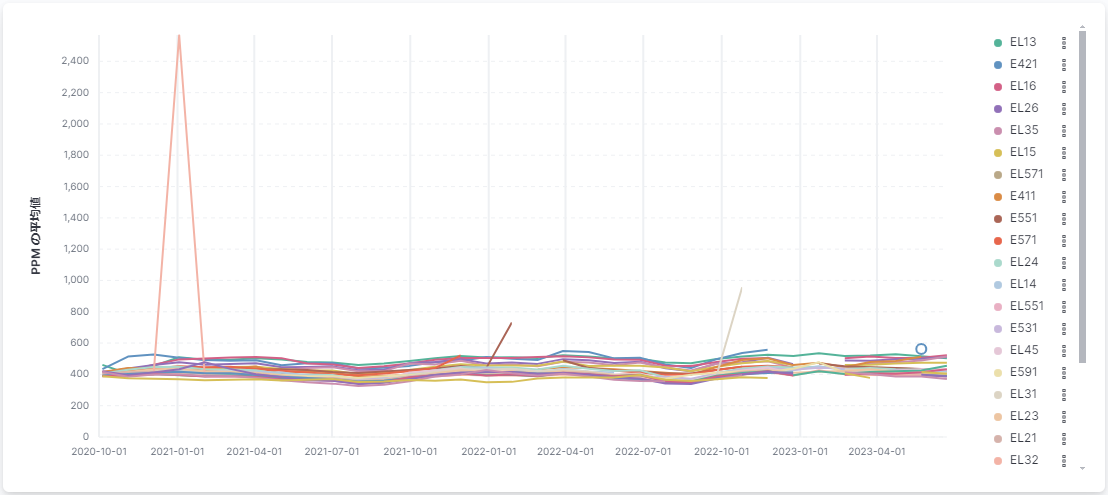
\includegraphics[width=170mm]{sotu/figure/ppm.png}
  \caption{co2\_modbusのPPM(30日間のPPMの平均値)}
  \label{p12}
\end{figure}

\begin{figure}[H]
  \hspace*{-2cm} % ここで左に2cmずらす
  \centering % center環境の代わりにこちらを使用
  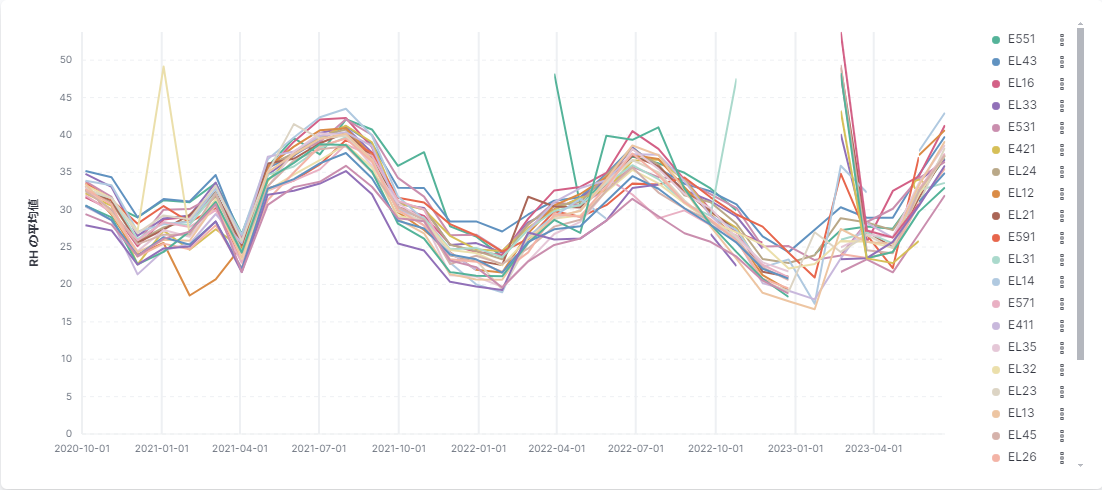
\includegraphics[width=170mm]{sotu/figure/rh.png}
  \caption{co2\_modbusのRH(30日間のRHの平均値)}
  \label{p13}
\end{figure}

\begin{figure}[H]
  \hspace*{-2cm} % ここで左に2cmずらす
  \centering % center環境の代わりにこちらを使用
  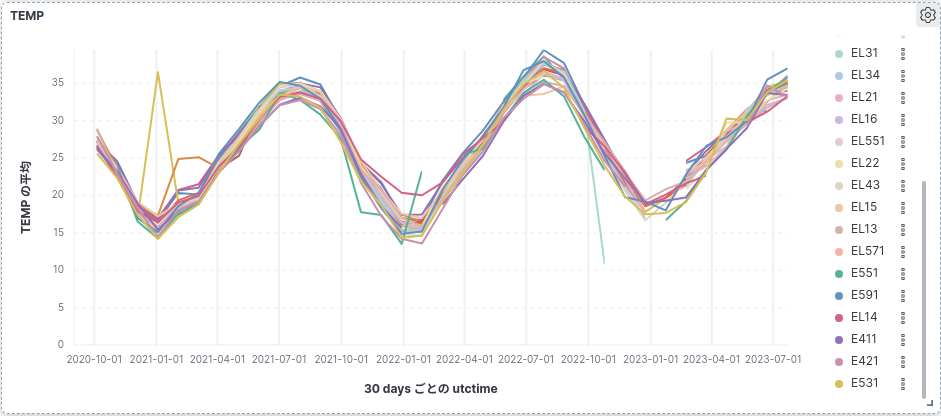
\includegraphics[width=170mm]{sotu/figure/temp.png}
  \caption{co2\_modbusの気温(30日間の気温の平均値)}
  \label{p14}
\end{figure}

図 \ref{p12} 〜 図 \ref{p14}より, 連続的にデータが変化していることが目視で確認できるので, データを欠落することなく重複データを削除出来たと判断した. なお, EL31教室にて気温が連続的に変化していないがこれはデータ計測システムが正常に動作せず計測出来ていなかったことが原因である. また, 2021年1月1日にE531教室の気温が他の教室より20℃程度高く計測されているが, これはセンサーの故障による誤った計測値であり, 連続的に変化しなくて良いデータである.

% \section{LEAFの運行日誌に関するデータの移行について}

\section{LEAFの運行日誌に関するデータの移行手順について}

movement\_diary01インデックスのデータ移行は, 同名のインデックスを移行先のElasticSearchサーバーに作成して, 作成したインデックスにデータを挿入することで行う.

\subsection{データのエクスポート}
移行元のElasticSearchサーバーのデータのローカルマシンへのエクスポートには, elasticdumpライブラリを使用して, movement\_diary01インデックスの全ドキュメントをJSON形式でエクスポートした.

\subsection{データのインポート}
pythonのelasticsearchライブラリを使用し, 移行先のElasticsearchにmovement\_diary01という名前のインデックスを作成して, エクスポートしたデータを全てインサートした.

\section{結言}
本章では単一ElasticsearchノードからElasticsearchクラスタへのデータ移行について述べた.

次章ではDockerによる仮想環境を使用したクラスタリング動作の可否の検証ついて述べる.